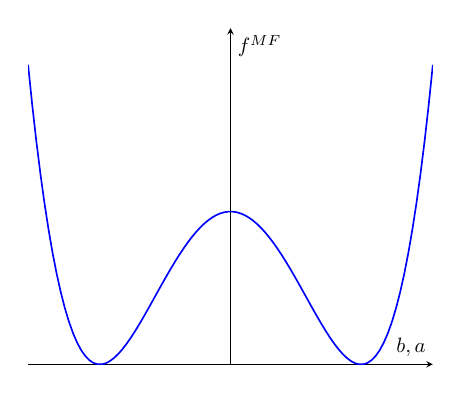
\begin{tikzpicture}[scale=0.75]
	\begin{axis}[
	ticks = none,
	xlabel = {$b,a$},
	ylabel = $f^{\text{MF}}$,
	x label style={at={(axis description cs:1,0.1)}, anchor = west},
	y label style={at={(axis description cs:0.15,1)},rotate=-90,anchor=south},
	ymax = 2,	
	axis lines = middle]
	
	
	
	\addplot[thick,
	domain=-2:2, 
	samples=100, 
	color=blue]{- x^2 + 0.3*x^4 + 1};
	
	\end{axis}
      %\draw[->] (-4,0) -- (4,0) node[right] {$b, a$};
      %\draw[->] (0,-4) -- (0,4) node[above] {$f^{MF}$};
      %\draw[blue] plot[samples=200,domain=-2:2] function {};
\end{tikzpicture}